\documentclass[12pt]{article}


\usepackage[english]{babel}
\usepackage[utf8]{inputenc}
\usepackage{amsmath,amssymb}
\usepackage{listings} % untuk kode python
\usepackage{xcolor}

\definecolor{codegreen}{rgb}{0,0.6,0}
\definecolor{codegray}{rgb}{0.5,0.5,0.5}
\definecolor{codepurple}{rgb}{0.58,0,0.82}
\definecolor{backcolour}{rgb}{0.95,0.95,0.92}

\lstdefinestyle{mystyle}{
    backgroundcolor=\color{backcolour},   
    commentstyle=\color{codegreen},
    keywordstyle=\color{magenta},
    numberstyle=\tiny\color{codegray},
    stringstyle=\color{codepurple},
    basicstyle=\ttfamily\footnotesize,
    breakatwhitespace=false,         
    breaklines=true,                 
    captionpos=b,                    
    keepspaces=true,                 
    numbers=left,                    
    numbersep=5pt,                  
    showspaces=false,                
    showstringspaces=false,
    showtabs=false,                  
    tabsize=2
}

\lstset{style=mystyle}
%\usepackage{parskip}
\usepackage{graphicx}

% Margins
\usepackage[top=2.5cm, left=3cm, right=3cm, bottom=4.0cm]{geometry}
\usepackage{hyperref}
\usepackage{natbib}
\usepackage{comment}
\usepackage{fancyvrb}
\setlength\bibsep{1em}
\setlength\bibhang{1.5em}
\renewcommand\bibfont{\singlespace}
\bibliographystyle{dcu}
% Colour table cells
%\usepackage[table]{xcolor}

% Get larger line spacing in table
\newcommand{\tablespace}{\\[1.25mm]}
\newcommand\Tstrut{\rule{0pt}{2.6ex}}         % = `top' strut
\newcommand\tstrut{\rule{0pt}{2.0ex}}         % = `top' strut
\newcommand\Bstrut{\rule[-0.9ex]{0pt}{0pt}}   % = `bottom' strut

%%%%%%%%%%%%%%%%%
%     Title     %
%%%%%%%%%%%%%%%%%
\title{Exercise 6 - Support Vector Machines}
\author{Azka NA}
\date{\today}

\begin{document}
\maketitle

%%%%%%%%%%%%%%%%%
%   Problem 1   %
%%%%%%%%%%%%%%%%%

\section{Introduction}
This is the guide for Andrew Ng's Machine Learning course programming assignment done in Python, adapted from the original guide written for Octave or MATLAB.

In this exercise, you will be using support vector machines (SVMs) to build a spam classifier. Before starting on the programming exercise, we strongly recommend completing the review questions for the associated topics.

For Programming Exercise 6: Support Vector Machines, you will need to download the following files:

\texttt{exercise6.ipynb} - Jupyter notebook containing the script

\texttt{ex6data1.mat} - Example Dataset 1

\texttt{ex6data2.mat} - Example Dataset 2

\texttt{ex6data3.mat} - Example Dataset 3

\texttt{spamTrain.mat} - Spam training set

\texttt{spamTest.mat} - Spam test set

\texttt{emailSample1.txt} - Sample email 1

\texttt{emailSample2.txt} - Sample email 2

\texttt{spamSample1.txt} - Sample spam 1

\texttt{spamSample2.txt} - Sample spam 2

\texttt{vocab.txt} - Vocabulary list

\hrulefill

\section{Support Vector Machines}

In the first half of this exercise, you will be using support vector machines (SVMs) with various example 2D datasets. Experimenting with these datasets will help you gain an intuition of how SVMs work and how to use a Gaussian kernel with SVMs.  In the next half of the exercise, you will be using support vector machines to build a spam classifier.

\subsection{Example Dataset 1}

We will begin by with a 2D example dataset which can be separated by a linear boundary.  You will plot the training data (Figure~\ref{fig:scatter}).  In this dataset, the positions of the positive examples (indicated with $+$) and the negative examples (indicated wit $o$) suggest a natural separation indicated by the gap.  However, notice that there is an outlier positive example $+$ on the far left at about (0.1,4.1).  As part of this exercise, you will also see how this outlier affects the SVM decision boundary.

\begin{figure}[h!]
  \centering
  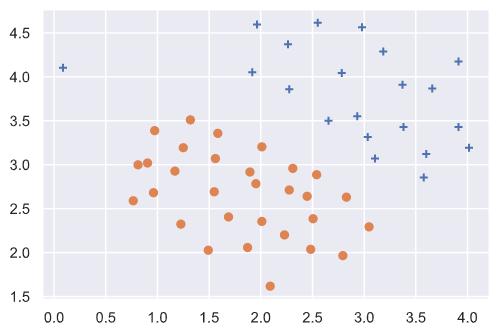
\includegraphics[scale=0.6]{scatter.png}
  \caption{Example Dataset 1}
  \label{fig:scatter}
\end{figure}

In this part of the exercise, you will try using different values of the $C$ parameter with SVMs.  Informally, the $C$ parameter is a positive value that controls the penalty for misclassified training examples.  A large $C$ parameter tells the SVM to try to classify all the examples correctly. $C$ plays a role similar to $\frac{1}{\lambda}$, where $\lambda$ is the regularization  parameter that we were using previously for logistic regression.

\begin{lstlisting}[language=Python]
from sklearn.svm import SVC
svc_cls = SVC(kernel='linear', C=1)
svc_cls.fit(X, y)
svc_cls.score(X, y)

pos = y==1
neg = y==0
plt.scatter(X[pos[:,0],0], X[pos[:,0],1], marker='+')
plt.scatter(X[neg[:,0],0], X[neg[:,0],1], marker='o')

# plotting the decision boundary
X_1,X_2 = np.meshgrid(np.linspace(X[:,0].min(),X[:,1].max(),num=100),np.linspace(X[:,1].min(),X[:,1].max(),num=100))

plt.contour(X_1,X_2, svc_cls.predict(np.array([X_1.ravel(),X_2.ravel()]).T).reshape(X_1.shape),1,colors='b')
\end{lstlisting}

\begin{figure}[h!]
  \centering
  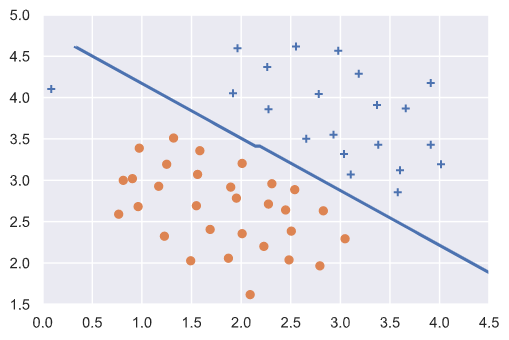
\includegraphics[scale=0.6]{c1.png}
  \caption{SVM Decision Boundary with $C$ = 1 (Example Dataset 1)}
  \label{fig:c1}
\end{figure}

\begin{figure}[h!]
  \centering
  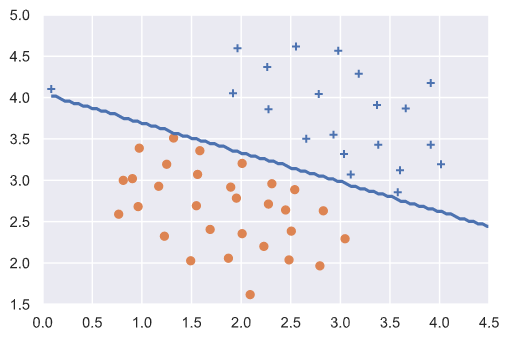
\includegraphics[scale=0.6]{c100.png}
  \caption{SVM Decision Boundary with $C$ = 100 (Example Dataset 1)}
  \label{fig:c100}
\end{figure}

The next part you will run the SVM training (with $C = 1$) using SVM module from `sklearn`.  When $C = 1$, you should find that the SVM puts the decision boundary in the gap between the two datasets and misclassifies the data point on the far left (Figure~\ref{fig:c1})

\framebox[14.5cm]{\parbox{14cm}{\textbf{Implementation Note:} Most SVM software packages automatically add the extra feature $x_0 = 1$ for you and automatically take care of learning the intercept term θ0. So when passing your training data to the SVM software, there is no need to add this extra feature $x_0 = 1$  yourself.}}

Your task is to try different values of $C$ on this dataset. Specifically, you should change the value of $C$ in the script to $C = 100$ and run the SVM training again. When $C = 100$, you should find that the SVM now classifies every single example correctly, but has a decision boundary that does not appear to be a natural fit for the data (Figure~\ref{fig:c100}).

\subsection{SVM with Gaussian Kernels}

In this part of the exercise, you will be using SVMs to do non-linear classification. In particular, you will be using SVMs with Gaussian kernels on datasets that are not linearly separable.

\subsubsection{Gaussian Kernel}

To find non-linear decision boundaries with the SVM, we need to first implement a Gaussian kernel. You can think of the Gaussian kernel as a similarity function that measures the "distance" between a pair of examples, $(x^{(i)}, x^{(j)})$. The Gaussian kernel is also parameterized by a bandwidth parameter, $\sigma$, which determines how fast the similarity metric decreases (to 0) as the examples are further apart.

You should now complete the code for \texttt{gaussianKernel} to compute the Gaussian kernel between two examples, $(x^{(i)}, x^{(j)})$. The Gaussian kernel function is defined as:

\begin{align}
  K_{gaussian}(x^{(i)}, x^{(j)}) = \text{exp} \bigg( -\frac{\|x^{(i)} - x^{(j)}\|^2}{2 \sigma^2} \bigg)
  = \text{exp} \Bigg(- \frac{\sum_{k=1}^n{(x_k^{(i)} - x_k^{(j)})^2}}{2 \sigma^2} \Bigg)
\end{align}

Once you’ve completed the function \texttt{gaussianKernel}, tou will test your kernel function on two provided examples and you should expect to see a value of 0.324652.

\begin{lstlisting}[language=Python]
def gaussianKernel(x1, x2, sigma):
    atas = np.sum((x1 - x2)**2)
    bawah = 2*(sigma**2)
    return np.exp(-atas/bawah)

x1 = np.array([1.0, 2.0, 1.0])
x2 = np.array([0.0, 4.0, -1.0])
sigma = 2
gaussianKernel(x1, x2, sigma)
\end{lstlisting}

\subsubsection{Example Dataset 2}

\begin{figure}[h!]
  \centering
  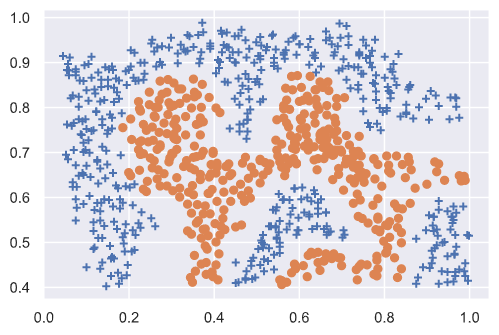
\includegraphics[scale=0.6]{scatter2.png}
  \caption{Example Dataset 2}
  \label{fig:scatter2}
\end{figure}

The next part you will load and plot dataset 2 (Figure\ref{fig:scatter2}). From the figure, you can observe that there is no linear decision boundary that separates the positive and negative examples for this dataset. However, by using the Gaussian kernel with the SVM, you will be able to learn a non-linear decision boundary that can perform reasonably well for the dataset.

\begin{lstlisting}[language=Python]
svc_cls3 = SVC(kernel='rbf', gamma=30)
svc_cls3.fit(X2, y2)
svc_cls3.score(X2, y2)
\end{lstlisting}


\begin{figure}[h!]
  \centering
  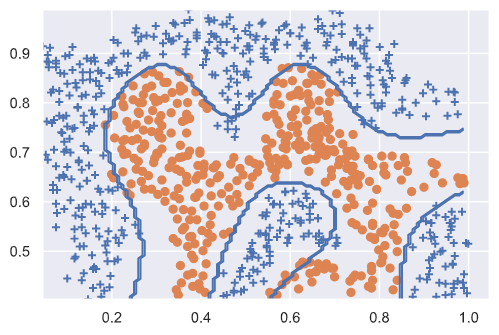
\includegraphics[scale=0.6]{boundary2.png}
  \caption{SVM (Gaussian Kernel) Decision Boundary (Example Dataset 2)}
  \label{fig:boundary2}
\end{figure}

Figure~\ref{fig:boundary2} shows the decision boundary found by the SVM with a Gaussian kernel. The decision boundary is able to separate most of the positive and negative examples correctly and follows the contours of the dataset well.

\subsubsection{Example Dataset 3}

In this part of the exercise, you will gain more practical skills on how to use a SVM with a Gaussian kernel. The next part you will load and display a third dataset (Figure~\ref{fig:scatter3}). You will be using the SVM with the Gaussian kernel with this dataset.

In the provided dataset, \texttt{ex6data3.mat}, you are given the variables \texttt{X, y, Xval, yval}. The provided code in ex6.m trains the SVM classifier using the training set (\texttt{X, y}) using parameters loaded from \texttt{dataset3Params}.

\begin{figure}[h!]
  \centering
  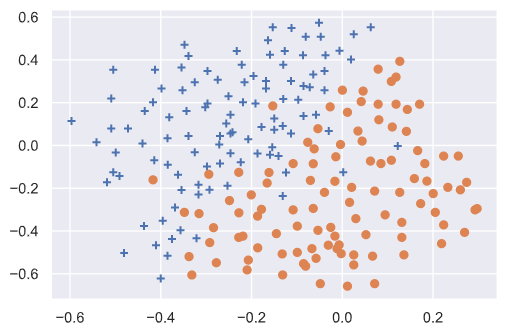
\includegraphics[scale=0.6]{scatter3.png}
  \caption{Example Dataset 3}
  \label{fig:scatter3}
\end{figure}

\begin{figure}[h!]
  \centering
  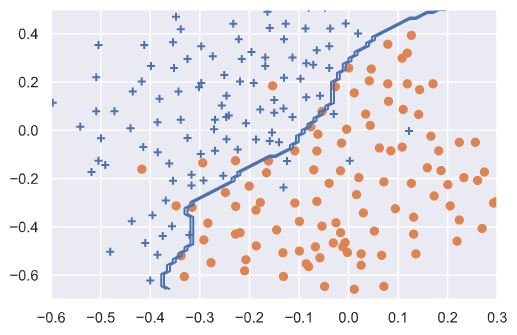
\includegraphics[scale=0.6]{boundary3.png}
  \caption{SVM (Gaussian Kernel) Decision Boundary (Example Dataset 3)}
  \label{fig:boundary3}
\end{figure}

Your task is to use the cross-validation set \texttt{Xval, yval} to determine the best $C$ and $\sigma$ parameter to use. You should write any additional code necessary to help you search over the parameters C and σ. For both $C$ and $\sigma$, we suggest trying values in multiplicative steps (e.g., 0.01, 0.03, 0.1, 0.3, 1, 3, 10, 30). Note that you should try all possible pairs of values for $C$ and $\sigma$ (e.g., $C = 0.3$ and $\sigma = 0.1$). For example, if you try each of the 8 values listed above for $C$ and for $\sigma^2$, you would end up training and evaluating (on the cross-validation set) a total of $8^2$ = 64 different models.

After you have determined the best $C$ and $\sigma$ parameters to use, you should modify the code in \texttt{dataset3Params}, filling in the best parameters you found. For our best parameters, the SVM returned a decision boundary shown in Figure~\ref{fig:boundary3}.

\begin{lstlisting}[language=Python]
def dataset3Params(X, y, Xval, yval, vals):
    best_score = 0
    best_params = {'C':None, 'gamma':None}

    for i in vals:
        C = i
        for j in vals:
            gamma = 1/j
            svc_cls = SVC(C=C, gamma=gamma)
            svc_cls.fit(X,y)
            prediction = svc_cls.predict(Xval)
            score = svc_cls.score(Xval, yval)
            if score > best_score:
                best_score = score
                best_params['C'] = C
                best_params['gamma'] = gamma
    return best_params['C'], best_params['gamma']
\end{lstlisting}

\hrulefill

\section{Spam Classification}

Many email services today provide spam filters that are able to classify emails into spam and non-spam email with high accuracy. In this part of the exercise, you will use SVMs to build your own spam filter.

You will be training a classifier to classify whether a given email, x, is spam ($y = 1$) or non-spam ($y = 0$). In particular, you need to convert each email into a feature vector $x \in \mathbb{R}^n$. The following parts of the exercise will walk you through how such a feature vector can be constructed from an email.

The dataset included for this exercise is based on a subset of the SpamAssassin Public Corpus.\footnote{\href{http://spamassassin.apache.org/old/publiccorpus/}{http://spamassassin.apache.org/old/publiccorpus/}} For the purpose of this exercise, you will only be using the body of the email (excluding the email headers).

\subsection{Preprocessing Emails}

\begin{figure}[h!]
  
  \framebox[15.5cm]{\parbox{15cm}{\texttt{
> Anyone knows how much it costs to host a web portal ?\\
>\\
Well, it depends on how many visitors youre expecting. This can be\\
anywhere from less than 10 bucks a month to a couple of \$100. You\\
should checkout http://www.rackspace.com/ or perhaps Amazon EC2 if\\
youre running something big..\\
\\
To unsubscribe yourself from this mailing list, send an email to:\\
groupname-unsubscribe@egroups.com}}}
  \caption{Sample Email}
  \label{block:sample}
  \end{figure}


Before starting on a machine learning task, it is usually insightful to take a look at examples from the dataset. Figure~\ref{block:sample} shows a sample email that contains a URL, an email address (at the end), numbers, and dollar amounts. While many emails would contain similar types of entities (e.g., numbers, other URLs, or other email addresses), the specific entities (e.g., the specific URL or specific dollar amount) will be different in almost every email. Therefore, one method often employed in processing emails is to  "normalize" these values, so that all URLs are treated the same, all numbers are treated the same, etc. For example, we could replace each URL in the email with the unique string "httpaddr" to indicate that a URL was present.

This has the effect of letting the spam classifier make a classification decision based on whether any URL was present, rather than whether a specific URL was present. This typically improves the performance of a spam classifier, since spammers often randomize the URLs, and thus the odds of seeing any particular URL again in a new piece of spam is very small.

In \texttt{processEmail}, we have implemented the following email preprocessing and normalization steps:

\begin{itemize}
  \item \textbf{Lower-casing:} The entire email is converted into lower case, so   that captialization is ignored (e.g., \texttt{IndIcaTE} is treated the same as   \texttt{Indicate}).
  \item \textbf{Stripping HTML:} All HTML tags are removed from the emails.   Many emails often come with HTML formatting; we remove all the   HTML tags, so that only the content remains.
  \item \textbf{Normalizing URLs:} All URLs are replaced with the text "\texttt{httpaddr}".
  \item \textbf{Normalizing Email Addresses:} All email addresses are replaced  with the text "\texttt{emailaddr}".
  \item \textbf{Normalizing Numbers:} All numbers are replaced with the text "\texttt{number}".
  \item \textbf{Normalizing Dollars:} All dollar signs (\$) are replaced with the text
  "\texttt{dollar}".
  \item \textbf{Word Stemming:} Words are reduced to their stemmed form. For example, "discount", "discounts", "discounted" and "discounting" are all   replaced with "\texttt{discount}". Sometimes, the Stemmer actually strips off additional characters from the end, so "include", "includes", "included", and "including" are all replaced with "\texttt{includ}".
  \item \textbf{Removal of non-words:} Non-words and punctuation have been removed. All white spaces (tabs, newlines, spaces) have all been trimmed to a single space character.
\end{itemize}

The result of these preprocessing steps is shown in Figure~\ref{block:preprocessed}. While preprocessing has left word fragments and non-words, this form turns out to be much easier to work with for performing feature extraction.

\begin{figure}[h!]
  
  \framebox[15.5cm]{\parbox{15cm}{\texttt{
anyon know how much it cost to host a web portal well it depend on \\
how mani visitor your expect thi can be anywher from less than\\
number buck a month to a coupl of dollarnumb you should\\
checkout httpaddr or perhap amazon ecnumb if your run someth big\\
to unsubscrib yourself from thi mail list send an email to \\ emailaddr}}}
  \caption{Preprocessed Sample Email}
  \label{block:preprocessed}
  \end{figure}

  \begin{figure}[hbt!]
    \centering
    %\subfloat[Vocabulary List]
    \framebox[4cm]{\parbox{3.5cm}{\texttt{1 aa
    2 ab \\
    3 abil \\
    ... \\
    86 anyon \\
    ... \\
    916 know \\
    ... \\
    1898 zero \\
    1899 zip}}}
      \caption{Vocabulary List}
    \label{fig:vocab}
  \end{figure}
   % \hfill
    %\subfloat[succinic acid]
  \begin{figure}[hbt!]
    \centering
    \framebox[5.5cm]{\parbox{5cm}{\texttt{86 916 794 1077 883 \\
    370 1699 790 1822 \\
    1831 883 431 1171 \\
    794 1002 1893 1364 \\
    592 1676 238 162 89 \\
    688 945 1663 1120 \\
    1062 1699 375 1162 \\
    479 1893 1510 799 \\
    1182 1237 810 1895 \\
    1440 1547 181 1699 \\
    1758 1896 688 1676 \\
    992 961 1477 71 530 \\
    1699 531}}}
    
      \caption{Word Indices for Sample Email}
    \label{fig:indices}
    %\caption{Cell growth and succinic acid titer for strain A and B in glass reactor under 3.5\% and 15\% \ce{O2} composition}
  \end{figure}

\subsubsection{Vocabulary List}

After preprocessing the emails, we have a list of words (e.g., Figure~\ref{block:preprocessed}) for each email. The next step is to choose which words we would like to use in our classifier and which we would want to leave out.

For this exercise, we have chosen only the most frequently occuring words as our set of words considered (the vocabulary list). Since words that occur rarely in the training set are only in a few emails, they might cause the model to overfit our training set. The complete vocabulary list is in the file \texttt{vocab.txt} and also shown in Figure~\ref{fig:vocab}. Our vocabulary list was selected by choosing all words which occur at least a 100 times in the spam corpus, resulting in a list of 1899 words. In practice, a vocabulary list with about 10,000 to 50,000 words is often used.

Given the vocabulary list, we can now map each word in the preprocessed emails (e.g., Figure~\ref{block:preprocessed}) into a list of word indices that contains the index of the word in the vocabulary list. Figure~\ref{fig:indices} shows the mapping for the sample email. Specifically, in the sample email, the word "anyone" was first normalized to "anyon" and then mapped onto the index 86 in the vocabulary list.

Your task now is to complete the code in \texttt{processEmail} to perform this mapping. In the code, you are given a string \texttt{str} which is a single word from the processed email. You should look up the word in the vocabulary list vocabList and find if the word exists in the vocabulary list. If the word exists, you should add the index of the word into the \texttt{word\_indices} variable. If the word does not exist, and is therefore not in the vocabulary, you can skip the word.

Once you have implemented processEmail.m, the script \texttt{ex6\_spam} will run your code on the email sample and you should see an output similar to Figures~\ref{block:preprocessed} &~\ref{fig:indices}.

\subsection{Extracting Features from Emails}

You will now implement the feature extraction that converts each email into a vector in $\mathbb{R}^n$. For this exercise, you will be using n = number of words in vocabulary list. Specifically, the feature $x_i \in \{0,1\}$ for an email corresponds to whether the $i$-th word in the dictionary occurs in the email. That is, $x_i = 1$ if the $i$-th word is in the email and $x_i = 0$ if the $i$-th word is not present in the email.

Thus, for a typical email, this feature would look like:

\begin{align}
  \mathbf x = \begin{bmatrix} 0 \\ \vdots  \\ 1 \\ 0 \\ \vdots  \\ 1 \\ 0 \\ \vdots \\ 0 \end{bmatrix} \in \mathbb{R}^n
\end{align}

You should now complete the code in \texttt{emailFeatures} to generate a feature vector for an email, given the \texttt{word\_indices}.

Once you have implemented \texttt{emailFeatures}, the next part of \texttt{ex6\_spam} will run your code on the email sample. You should see that the feature vector had length 1899 and 45 non-zero entries.

\subsection{Training SVM for Spam Classification}

After you have completed the feature extraction functions, the next step of \texttt{ex6\_spam} will load a preprocessed training dataset that will be used to train a SVM classifier. \texttt{spamTrain} contains 4000 training examples of spam and non-spam email, while \texttt{spamTest} contains 1000 test examples. Each original email was processed using the \texttt{processEmail} and \texttt{emailFeatures} functions and converted into a vector $x^{(i)} \in \mathbb{R}^{1899}$.

After loading the dataset, \texttt{ex6\_spam} will proceed to train a SVM to classify between spam ($y = 1$) and non-spam ($y = 0$) emails. Once the training completes, you should see that the classifier gets a training accuracy of about 99.8\% and a test accuracy of about 98.5\%.

\subsection{Top Predictors for Spam}


\begin{figure}[h!]
  
  \framebox[15.5cm]{\parbox{15cm}{\texttt{
    our click remov guarante visit basenumb dollar will price pleas \\ 
    nbsp most lo ga dollarnumb}}}
  \caption{Top predictors for spam email}
  \label{block:predictors}
  \end{figure}

  To better understand how the spam classifier works, we can inspect the parameters to see which words the classifier thinks are the most predictive of spam. The next step of ex6 spam.m finds the parameters with the largest positive values in the classifier and displays the corresponding words (Figure~\ref{block:predictors}). Thus, if an email contains words such as "guarantee", "remove", "dollar", and "price" (the top predictors shown in Figure~\ref{block:predictors}), it is likely to be classified as spam.

\subsection{Optional (ungraded) exercise: Try your own emails}

Now that you have trained a spam classifier, you can start trying it out on your own emails. In the starter code, we have included two email examples (\texttt{emailSample1.txt} and \texttt{emailSample2.txt}) and two spam examples (\texttt{spamSample1.txt} and \texttt{spamSample2.txt}). The last part of ex6 spam.m runs the spam classifier over the first spam example and classifies it using the learned SVM. You should now try the other examples we have provided and see if the classifier gets them right. You can also try your own emails by replacing the examples (plain text files) with your own emails. 

\subsection{Optional (ungraded) exercise: Build your own dataset}

In this exercise, we provided a preprocessed training set and test set. These datasets were created using \texttt{processEmail} and \texttt{emailFeatures} that you now have completed. For this optional (ungraded) exercise, you will build your own dataset using the original emails from the \href{http://spamassassin.apache.org/old/publiccorpus/}{SpamAssassin Public Corpus}.

Your task in this optional (ungraded) exercise is to download the original files from the public corpus and extract them. After extracting them, you should run the \texttt{processEmail}\footnote{The original emails will have email headers that you might wish to leave out. We have included code in \texttt{processEmail} that will help you remove these headers.} and \texttt{emailFeatures} functions on each email to extract a feature vector from each email. This will allow you to build a dataset \texttt{X, y} of examples. You should then randomly divide up the dataset into a training set, a cross-validation set and a test set.

While you are building your own dataset, we also encourage you to try building your own vocabulary list (by selecting the high frequency words that occur in the dataset) and adding any additional features that you think might be useful.

\begin{comment}
\section{Introduction}
This is the guide for Andrew Ng's Machine Learning course programming assignment done in Python, adapted from the original guide written for Octave or MATLAB.

In this exercise, you will implement regularized linear regression and use it to study models with different bias-variance properties. Before starting on this programming exercise, we strongly recommend watching the video lectures and completing the review questions for the associated topics

For Programming Exercise 5: Regularized Linear Regression and Bias v.s. Variance, you will need to download the following files:

\texttt{exercise5.ipynb} - Jupyter notebook containing the script

\texttt{ex5data1.mat} - Dataset

\hrulefill

\section{Regularized Linear Regression}

In the first half of the exercise, you will implement regularized linear regression to predict the amount of water flowing out of a dam using the change of water level in a reservoir. In the next half, you will go through some diagnostics of debugging learning algorithms and examine the effects of bias v.s. variance.

\subsection{Visualizing the dataset}

We will begin by visualizing the dataset containing historical records on the change in the water level, $x$, and the amount of water flowing out of the dam, $y$, as shown in Figure~\ref{fig:scatter}

This dataset is divided into three parts:

\begin{itemize}
  \item A \textbf{training} set that your model will learn on: \texttt{X, y}
  \item A \textbf{cross validation} set for determining the regularization parameter: \texttt{Xval, yval}
  \item A \textbf{test} set for evaluating performance. These are "unseen" examples which your model did not see during training: \texttt{Xtest, ytest}
\end{itemize}

In the following parts, you will implement linear regression and use that to fit a straight line to the data and plot learning curves. Following that, you will implement polynomial regression to find a better fit to the data.

\begin{figure}[h!]
  \centering
  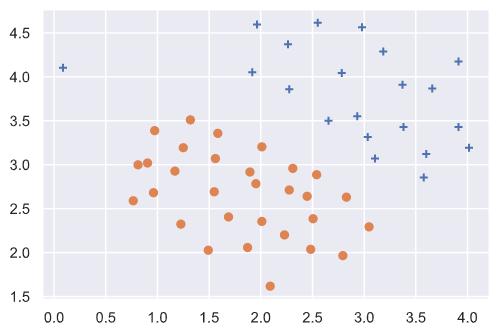
\includegraphics[scale=0.6]{scatter.png}
  \caption{Data}
  \label{fig:scatter}
\end{figure}

\subsection{Regularized linear regression cost function}
Recall that regularized linear regression has the following cost function:

\begin{align}
  J(\theta_1) & = \frac{1}{2m}\Big(\sum_{i=1}^m{(h_\theta(x^{(i)})-y^{(i)})^2}\Big) + \frac{\lambda}{2m}\Big(\sum_{j=1}^n{{\theta_j}^2}\Big),
\end{align}

where $\lambda$ is a regularization parameter which controls the degree of regularization (thus, help preventing overfitting). The regularization term puts a penalty on the overall cost $J$. As the magnitudes of the model parameters $\theta_j$ increase, the penalty increases as well. Note that you should not regularize the $\theta_0$ term.

Your task is to write a function to calculate the regularized linear regression cost function. If possible, try to vectorize your code and avoid writing loops.

\begin{lstlisting}[language=Python]
  def linearRegCostFunction(X, y, theta, Lambda):
    m = len(y)
    y = y.reshape(m,1)
    grad = np.zeros(theta.shape)
    n_1 = theta.shape[0]
    theta = theta.reshape(n_1,1)
    cost = 0
    h = np.dot(X, theta)
    cost = 1/(2*m) * np.sum((h-y)**2)
    cost_reg = cost + Lambda/(2*m)*np.sum(theta[1:]**2)

    grad[0] = (1/m)*(X[:,0:1].reshape(m,1)*(h - y)).sum(axis=0)
    grad[1:] = (1/m)*( (X[:,1:]*(h - y)).sum(axis=0)  + Lambda*theta[1:].reshape(n_1-1))

    return cost_reg, grad
\end{lstlisting}

When you are finished, run your cost function using \texttt{theta} initialized at \texttt{[1,1]}. You should expect to see an output of 303.993.

\subsection{Regularized linear regression gradient}

Correspondingly, the partial derivative of regularized linear regression's cost for $\theta_j$ is defined as

\begin{align}
  \frac{\partial J(\theta)}{\partial \theta_0} & = \frac{1}{m}\sum_{i=1}^m{(h_\theta(x^{(i)})-y^{(i)}) x_j^{(i)}} & \text{for} j & = 0 \\
  \frac{\partial J(\theta)}{\partial \theta_j} & = \bigg(\frac{1}{m}\sum_{i=1}^m{(h_\theta(x^{(i)})-y^{(i)}) x_j^{(i)}}\bigg) + \frac{\lambda}{m}\theta_j & \text{for} j & \geq 1
\end{align}


Run your cost function using theta initialized at [1,1]. You should expect to see a gradient of \texttt{[-15.30, 598.250]}.

\subsection{Fitting linear regression}

Once your cost function and gradient are working correctly, compute the optimal values of $\theta$ using the \texttt{minimize} function from Scipy's \texttt{Optimize} module.

In this part, we set regularization parameter $\lambda$ to zero. Because our current implementation of linear regression is trying to fit a 2-dimensional $\theta$, regularization will not be incredibly helpful for a $\theta$ of such low dimension. In the later parts of the exercise, you will be using polynomial regression with regularization.

\begin{lstlisting}[language=Python]
  def trainLinearReg(linearRegCostFunction, X, y, Lambda=0, maxiter=200):

    initial_theta = np.zeros(X.shape[1])
    costFunction = lambda t: linearRegCostFunction(X, y, t, Lambda)
    options = {'maxiter': maxiter}
    minimizef = optimize.minimize(costFunction, initial_theta, jac=True, method='TNC', options=options)
    return minimizef.x 
\end{lstlisting}

Finally, we should also plot the best fit line, resulting in an image similar to Figure ~\ref{fig:linearfit}. The best fit line tells us that the model is not a good fit to the data because the data has a non-linear pattern. While visualizing the best fit as shown is one possible way to debug your learning algorithm, it is not always easy to visualize the data and model. In the next section, you will implement a function to generate learning curves that can help you debug your learning algorithm even if it is not easy to visualize the data.

\begin{figure}[h!]
  \centering
  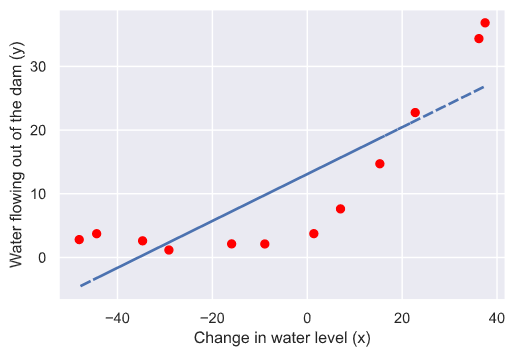
\includegraphics[scale=0.6]{linearfit.png}
  \caption{Linear fit}
  \label{fig:linearfit}
\end{figure}

\section{Bias-variance}

An important concept in machine learning is the bias-variance tradeoff. Models with high bias are not complex enough for the data and tend to underfit, while models with high variance overfit to the training data.

In this part of the exercise, you will plot training and test errors on a learning curve to diagnose bias-variance problems.

\subsection{Learning curves}

You will now implement code to generate the learning curves that will be useful in debugging learning algorithms. Recall that a learning curve plots training and cross-validation error as a function of training set size. Your job is to write a function so that it returns a vector of errors for the training set and cross-validation set.

To plot the learning curve, we need a training and cross-validation set error for different training set sizes. To obtain different training set sizes, you should use different subsets of the original training set \texttt{X}. Specifically, for a training set size of i, you should use the first i examples (i.e., \texttt{X[:i,:]} and \texttt{y[:i]}).

You can use the \texttt{trainLinearReg} function to find the $\theta$ parameters. Note that the lambda is passed as a parameter to the \texttt{learningCurve} function. After learning the $\theta$ parameters, you should compute the \textbf{error} on the training and cross-validation sets. Recall that the training error for a dataset is defined as

\begin{align}
  J(\theta_1) & = \frac{1}{2m}\bigg[\sum_{i=1}^m{(h_\theta(x^{(i)})-y^{(i)})^2}\bigg].
\end{align}

In particular, note that the training error does not include the regularization term. One way to compute the training error is to use your existing cost function and set $\lambda$ to 0 only when using it to compute the training error and cross-validation error. When you are computing the training set error, make sure you compute it on the training subset (i.e., \texttt{X[:n]} and \texttt{y[:n]}) (instead of the entire training set). However, for the cross-validation error, you should compute it over the entire cross-validation set. You should store the computed errors in the vectors \texttt{training\_error} and \texttt{validation\_error}.

\begin{lstlisting}[language=Python]
  def learningCurve(X, y, Xval, yval, Lambda=0):
    m = len(y)
    training_error = np.zeros(m)
    validation_error = np.zeros(m)

    for i in range(m):
        theta_optimized1 = trainLinearReg(linearRegCostFunction, X[:i+1], y[:i+1], Lambda)
        training_error[i], _ = linearRegCostFunction(X[:i+1], y[:i+1], theta_optimized1, Lambda)
        validation_error[i], _ = linearRegCostFunction(Xval, yval, theta_optimized1, Lambda)

    return training_error, validation_error
\end{lstlisting}

When you are finished, print the learning curves and make a plot similar to Figure~\ref{fig:learningcurve}.

\begin{figure}[h!]
  \centering
  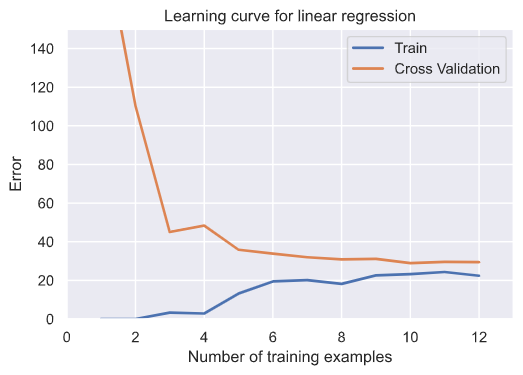
\includegraphics[scale=0.6]{learningcurve.png}
  \caption{Linear regression learning curve}
  \label{fig:learningcurve}
\end{figure}

In Figure~\ref{fig:learningcurve}, you can observe that both the train error and cross-validation error are high when the number of training examples is increased. This reflects a \textbf{high bias} problem in the model --- the linear regression model is too simple and is unable to fit our dataset well. In the next section, you will implement polynomial regression to fit a better model for this dataset.

\section{Polynomial regression}

The problem with our linear model was that it was too simple for the data and resulted in underfitting (high bias). In this part of the exercise, you will address this problem by adding more features.

For use polynomial regression, our hypothesis has the form:

\begin{align}
  h_\theta(x) & = \theta_0 + \theta_1 * (\text{waterLevel}) + \theta_2 * (\text{waterLevel})^2 + \dots + \theta_p * (\text{waterLevel})^p \\
   & = \theta_0 + \theta_1 x_1 + \theta_2 x_2 + \dots + \theta_p x_p 
\end{align}

Notice that by defining $x_1 = \text{(waterLevel)}$, $x_2 = \text{(waterLevel)}^2$, $\dots$, $x_p = \text{(waterLevel)}^p$, we obtain a linear regression model where the features are the various powers of the original value (waterLevel).

Now, you will add more features using the higher powers of the existing feature $x$ in the dataset. Your task in this part is to complete the code for \texttt{polyFeatures} so that the function maps the original training set \texttt{X} of size $m \times 1$ into its higher powers. Specifically, when a training set \texttt{X} of size $m \times 1$ is passed into the function, the function should return a $m \times p$ matrix \texttt{X\_poly}, where column 1 holds the original values of \texttt{X}, column 2 holds the values of $\verb!X.^2!$, column 3 holds the values of $\verb!X.^3!$, and so on. Note that you don’t have to account for the zero-eth power in this function.

\begin{lstlisting}[language=Python]
  def polyFeatures(X, p):
    m = X.shape[0]
    X_out = np.zeros((m,p))
    for i in range(p):
        X_out[:,i] = X.flatten()**(i+1)
    return X_out
\end{lstlisting}


Now you have a function that will map features to a higher dimension, then apply it to the training set, the test set, and the cross-validation set (which you haven’t used yet).

\subsection{Learning Polynomial Regression}

After you have completed \texttt{polyFeatures}, we will proceed to train polynomial regression using your linear regression cost function.

Keep in mind that even though we have polynomial terms in our feature vector, we are still solving a linear regression optimization problem. The polynomial terms have simply turned into features that we can use for linear regression. We are using the same cost function and gradient that you wrote for the earlier part of this exercise.

For this part of the exercise, you will be using a polynomial of degree 8. It turns out that if we run the training directly on the projected data, will not work well as the features would be badly scaled (e.g., an example with $x = 40$ will now have a feature $x_8 = 40^8 = 6.5 \times 10^{12}$). Therefore, you will need to use feature normalization.

Before learning the parameters $\theta$ for the polynomial regression, we will first call \texttt{featureNormalize} and normalize the features of the training set, storing the mu, sigma parameters separately. 

After learning the parameters $\theta$, you should see two plots (Figure~\ref{fig:polynomialfit},\ref{fig:polylearningcurve}) generated for polynomial regression with $\lambda = 0$.

\begin{figure}[h!]
  \centering
  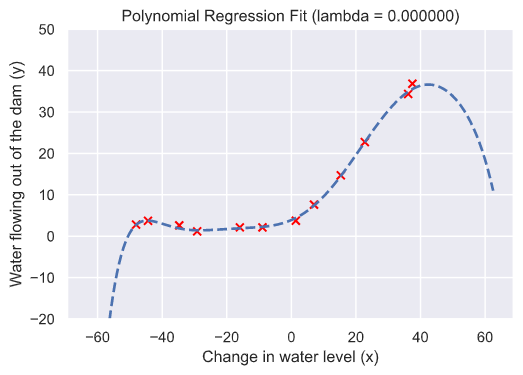
\includegraphics[scale=0.6]{polynomialfit.png}
  \caption{Polynomial fit, $\lambda = 0$}
  \label{fig:polynomialfit}
\end{figure}

\begin{figure}[h!]
  \centering
  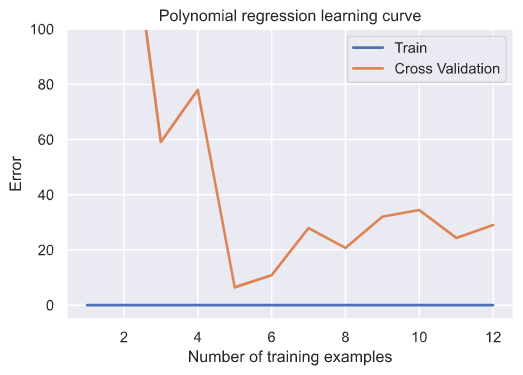
\includegraphics[scale=0.6]{polylearningcurve.png}
  \caption{Polynomial learning curve, $\lambda = 0$}
  \label{fig:polylearningcurve}
\end{figure}

From Figure ~\ref{fig:polynomialfit}, you should see that the polynomial fit is able to follow the datapoints very well - thus, obtaining a low training error. However, the polynomial fit is very complex and even drops off at the extremes. This is an indicator that the polynomial regression model is overfitting the training data and will not generalize well.

To better understand the problems with the unregularized ($\lambda = 0$) model, you can see that the learning curve (Figure~\ref{fig:polylearningcurve}) shows the same effect where the low training error is low, but the cross validation error is high. There
is a gap between the training and cross validation errors, indicating a high
variance problem.

One way to combat the overfitting (high-variance) problem is to add regularization to the model. In the next section, you will get to try different $\lambda$ parameters to see how regularization can lead to a better model.

\subsection{Optional (ungraded) exercise: Adjusting the regularization parameter}

In this section, you will get to observe how the regularization parameter affects the bias-variance of regularized polynomial regression. You should now modify the the \texttt{Lambda} parameter and try $\lambda = 1, 100$. For each of these values, the script should generate a polynomial fit to the data and also a learning curve.

For $\lambda = 1$, you should see a polynomial fit that follows the data trend well (Figure~\ref{fig:polyfit1}) and a learning curve (Figure~\ref{fig:polycurve1}) showing that both the cross-validation and training error converge to a relatively low value. This shows the $\lambda = 1$ regularized polynomial regression model does not have the highbias or high-variance problems. In effect, it achieves a good trade-off between bias and variance.

For $\lambda = 100$, you should see a polynomial fit (Figure~\ref{fig:polyfit100}) that does not follow the data well. In this case, there is too much regularization and the model is unable to fit the training data.

\begin{figure}[h!]
  \centering
  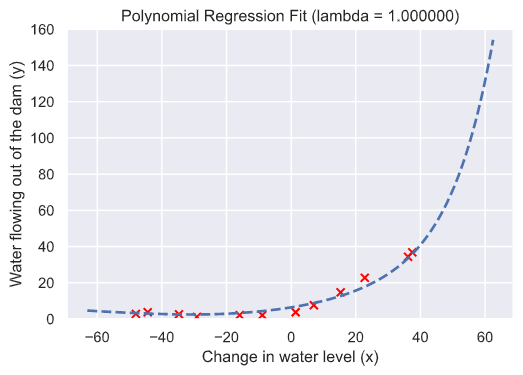
\includegraphics[scale=0.6]{polyfit1.png}
  \caption{Polynomial fit, $\lambda = 1$}
  \label{fig:polyfit1}
\end{figure}

\begin{figure}[h!]
  \centering
  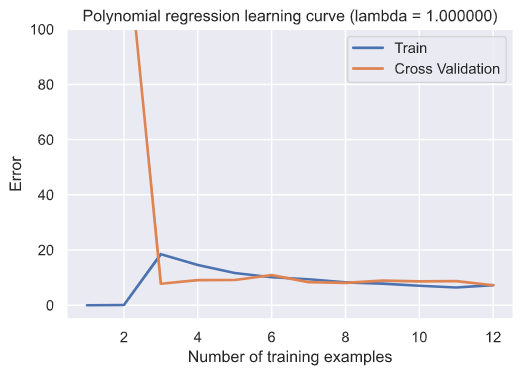
\includegraphics[scale=0.6]{polycurve1.png}
  \caption{Polynomial learning curve, $\lambda = 1$}
  \label{fig:polycurve1}
\end{figure}

\begin{figure}[h!]
  \centering
  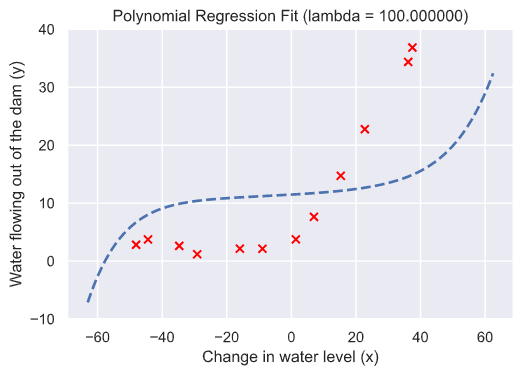
\includegraphics[scale=0.6]{polyfit100.png}
  \caption{Polynomial fit, $\lambda = 100$}
  \label{fig:polyfit100}
\end{figure}

\subsection{Selecting $\lambda$ using a cross validation set}

From the previous parts of the exercise, you observed that the value of $\lambda$ can significantly affect the results of regularized polynomial regression on the training and cross-validation set. In particular, a model without regularization ($\lambda = 0$) fits the training set well, but does not generalize. Conversely, a model with too much regularization ($\lambda = 100$) does not fit the training set and testing set well. A good choice of $\lambda$ (e.g., $\lambda = 1$) can provide a good fit to the data.

In this section, you will implement an automated method to select the $\lambda$ parameter. Concretely, you will use a cross-validation set to evaluate how good each $\lambda$ value is. After selecting the best $\lambda$ value using the cross-validation set, we can then evaluate the model on the test set to estimate how well the model will perform on actual unseen data.

Your task is to complete the code for \texttt{validationCurve}. Specifically, you should should use the \texttt{trainLinearReg} function to train the model using different values of $\lambda$ and compute the training error and cross-validation error. You should try $\lambda$ in the following range: \{0, 0.001, 0.003, 0.01, 0.03, 0.1, 0.3, 1, 3, 10\}.

\begin{lstlisting}[language=Python]
  def validationCurve(X, y, Xval, yval):
    
    lambda_vec = [0, 0.001, 0.003, 0.01, 0.03, 0.1, 0.3, 1, 3, 10]

    training_error = np.zeros(len(lambda_vec))
    validation_error = np.zeros(len(lambda_vec))

    for i in range(len(lambda_vec)):
      lambda_try = lambda_vec[i]
      theta_t = trainLinearReg(linearRegCostFunction, X, y, Lambda = lambda_try)
      training_error[i], _ = linearRegCostFunction(X, y, theta_t, Lambda = 0)
      validation_error[i], _ = linearRegCostFunction(Xval, yval, theta_t, Lambda = 0)

    return lambda_vec, training_error, validation_error
\end{lstlisting}

\begin{figure}[h!]
  \centering
  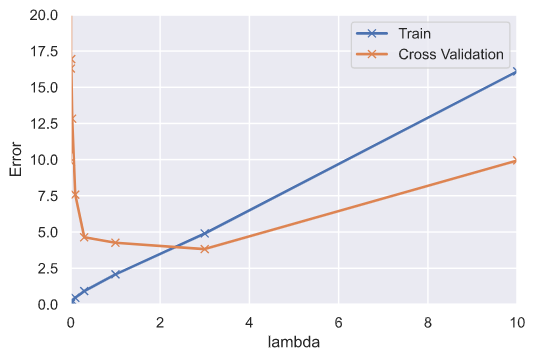
\includegraphics[scale=0.6]{selectlambda.png}
  \caption{Selecting $\lambda$ using a cross-validation set}
  \label{fig:selectlambda}
\end{figure}

After you have completed the code, run your function to plot a cross-validation curve of error v.s. $\lambda$ that allows you select which $\lambda$ parameter to use. You should see a plot similar to Figure ~\ref{fig:selectlambda}. In this figure, we can see that the best value of $\lambda$ is around 3. Due to randomness in the training and validation splits of the dataset, the cross-validation error can sometimes be lower than the training error.

\subsection{Optional (ungraded) exercise: Computing test set error}

In the previous part of the exercise, you implemented code to compute the cross-validation error for various values of the regularization parameter $\lambda$. However, to get a better indication of the model’s performance in the real world, it is important to evaluate the "final" model on a test set that was not used in any part of training (that is, it was neither used to select the $\lambda$ parameters, nor to learn the model parameters $\theta$).

For this optional (ungraded) exercise, you should compute the test error
using the best value of $\lambda$ you found. In our cross validation, we obtained a
test error of 3.8599 for $\lambda= 3$ .

\subsection{Optional (ungraded) exercise: Plotting learning curves with randomly selected examples}

In practice, especially for small training sets, when you plot learning curves to debug your algorithms, it is often helpful to average across multiple sets of randomly selected examples to determine the training error and cross validation error.

Concretely, to determine the training error and cross validation error for $i$ examples, you should first randomly select $i$ examples from the training set and $i$ examples from the cross validation set. You will then learn the parameters $\theta$ using the randomly chosen training set and evaluate the parameters $\theta$ on the randomly chosen training set and cross validation set. The above steps should then be repeated multiple times (say 50) and the averaged error should be used to determine the training error and cross validation error for $i$ examples.
\end{comment}

\end{document}
